\documentclass[pdflatex,compress,mathserif]{beamer}

%\usetheme[dark,framenumber,totalframenumber]{ElektroITK}
\usetheme[darktitle,framenumber,totalframenumber]{ElektroITK}

\usepackage[utf8]{inputenc}
\usepackage[T1]{fontenc}
\usepackage{lmodern}
\usepackage[bahasai]{babel}
\usepackage{amsmath}
\usepackage{amsfonts}
\usepackage{amssymb}
\usepackage{graphicx}
\usepackage{multicol}
\usepackage{lipsum}

\newcommand*{\Scale}[2][4]{\scalebox{#1}{$#2$}}%

\title{Sinyal dan Sistem}
\subtitle{Sistem}

\author{Mifta Nur Farid}

\begin{document}

% ----------------------------------------------------------------------------
% *** Titlepage <<<
% ----------------------------------------------------------------------------
\maketitle
% ----------------------------------------------------------------------------
% *** END of Titlepage >>>
% ----------------------------------------------------------------------------

\section{Definisi Sistem}
\begin{frame}{Definisi Sistem}
	\begin{figure}
		\centering
		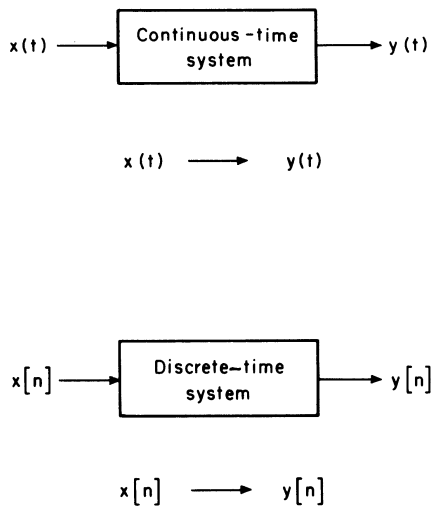
\includegraphics[height=0.8\textheight]{img/02.slide_09}
	\end{figure}
\end{frame}

\section{Interkoneksi Antar Sistem}
\begin{frame}{Interkoneksi Antar Sistem}
	\begin{figure}
		\centering
		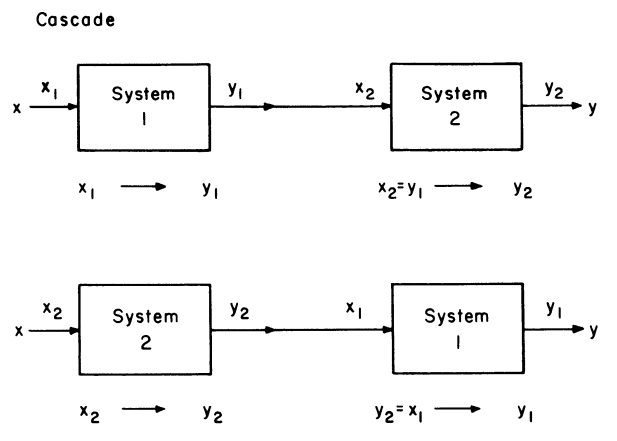
\includegraphics[height=0.8\textheight]{img/02.slide_10}
	\end{figure}
\end{frame}

\begin{frame}{Interkoneksi Antar Sistem}
	\begin{figure}
		\centering
		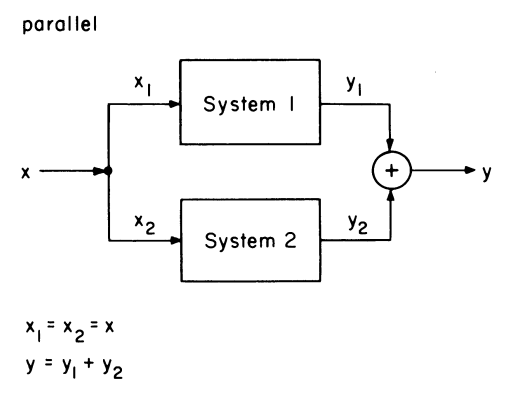
\includegraphics[height=0.8\textheight]{img/02.slide_11}
	\end{figure}
\end{frame}

\begin{frame}{Interkoneksi Antar Sistem}
	\begin{figure}
		\centering
		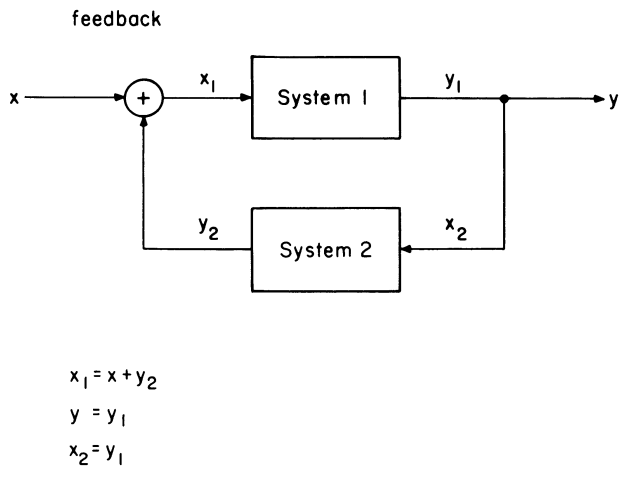
\includegraphics[height=0.8\textheight]{img/02.slide_12}
	\end{figure}
\end{frame}

\section{Karakteristik Sistem}
\begin{frame}{Karakteristik Sistem}
	\begin{figure}
		\centering
		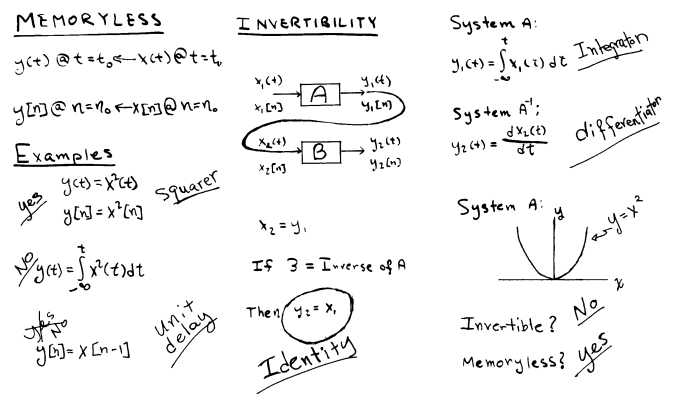
\includegraphics[height=0.8\textheight]{img/02.slide_13}
	\end{figure}
\end{frame}

\begin{frame}{Karakteristik Sistem}
	\begin{figure}
		\centering
		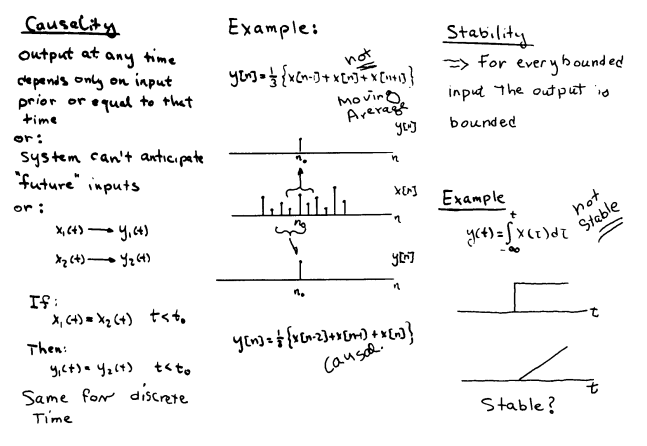
\includegraphics[height=0.85\textheight]{img/02.slide_14}
	\end{figure}
\end{frame}

\begin{frame}{Karakteristik Sistem}
	\begin{figure}
		\centering
		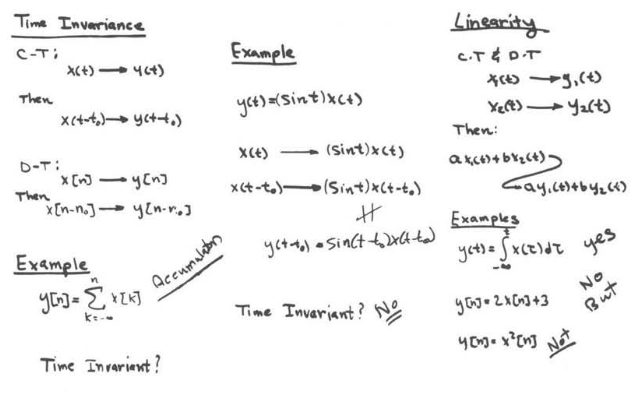
\includegraphics[height=0.85\textheight]{img/02.slide_15}
	\end{figure}
\end{frame}

\end{document}
